\clearpage
\subsection{Assignment Statement (with Fields and Elements)} % (fold)
\label{sub:assignment_statement_with_fields_and_elements_}

The Assignment Statement allows you to store a value in a Variable or Array. The righthand side of the assignment is an expression that calculates the value to be stored. The lefthand side is a variable or array element, a place into which the value can be stored. With the addition of the custom types you can now also store values in \textbf{fields} of a record or union.

\begin{figure}[h]
   \centering
   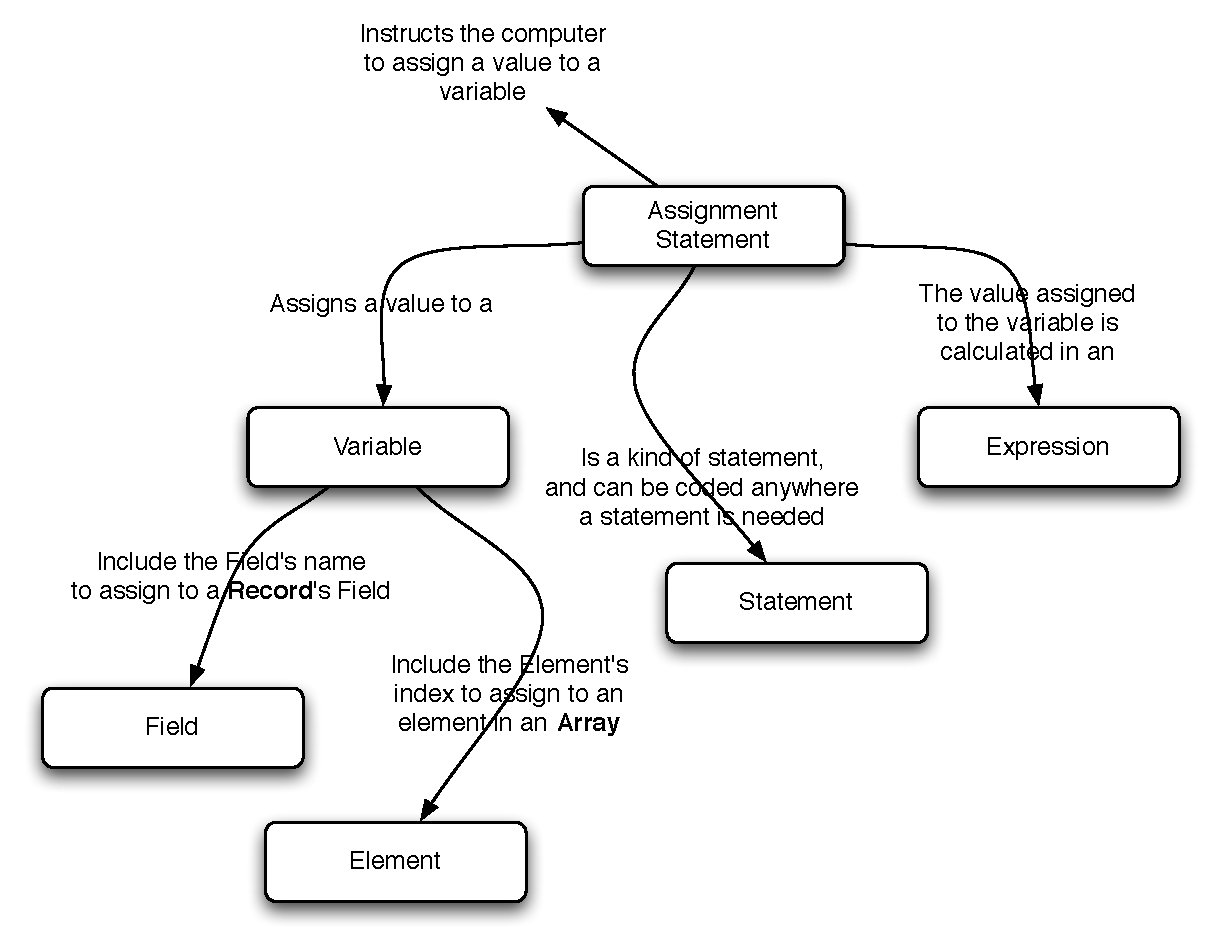
\includegraphics[width=\textwidth]{./topics/type-decl/diagrams/Assignment} 
   \caption{You can assign values to a Record or Union's fields}
   \label{fig:type-decl-assignment}
\end{figure}

\mynote{
\begin{itemize}
  \item The Assignment Statement is an \textbf{action}, you can command the computer to store a value in a variable, array element, record's field, or union's field.
  \item Enumeration values are stored in a single variable, so they work in the same way as shown in \sref{sub:assignment_statement} \nameref{sub:assignment_statement}.
  \item With a record you can assign values to its fields individually, or you can assign it all of the values from another matching record.
  \item A union can have its value set via its fields, or you can copy the value from another matching union.
\end{itemize}
}

\clearpage
\subsubsection{Record Assignment} % (fold)
\label{ssub:record_assignment}

The assignment statement can be used to assign a value to a record's fields, or to copy an existing record's values.

\begin{figure}[h]
   \centering
   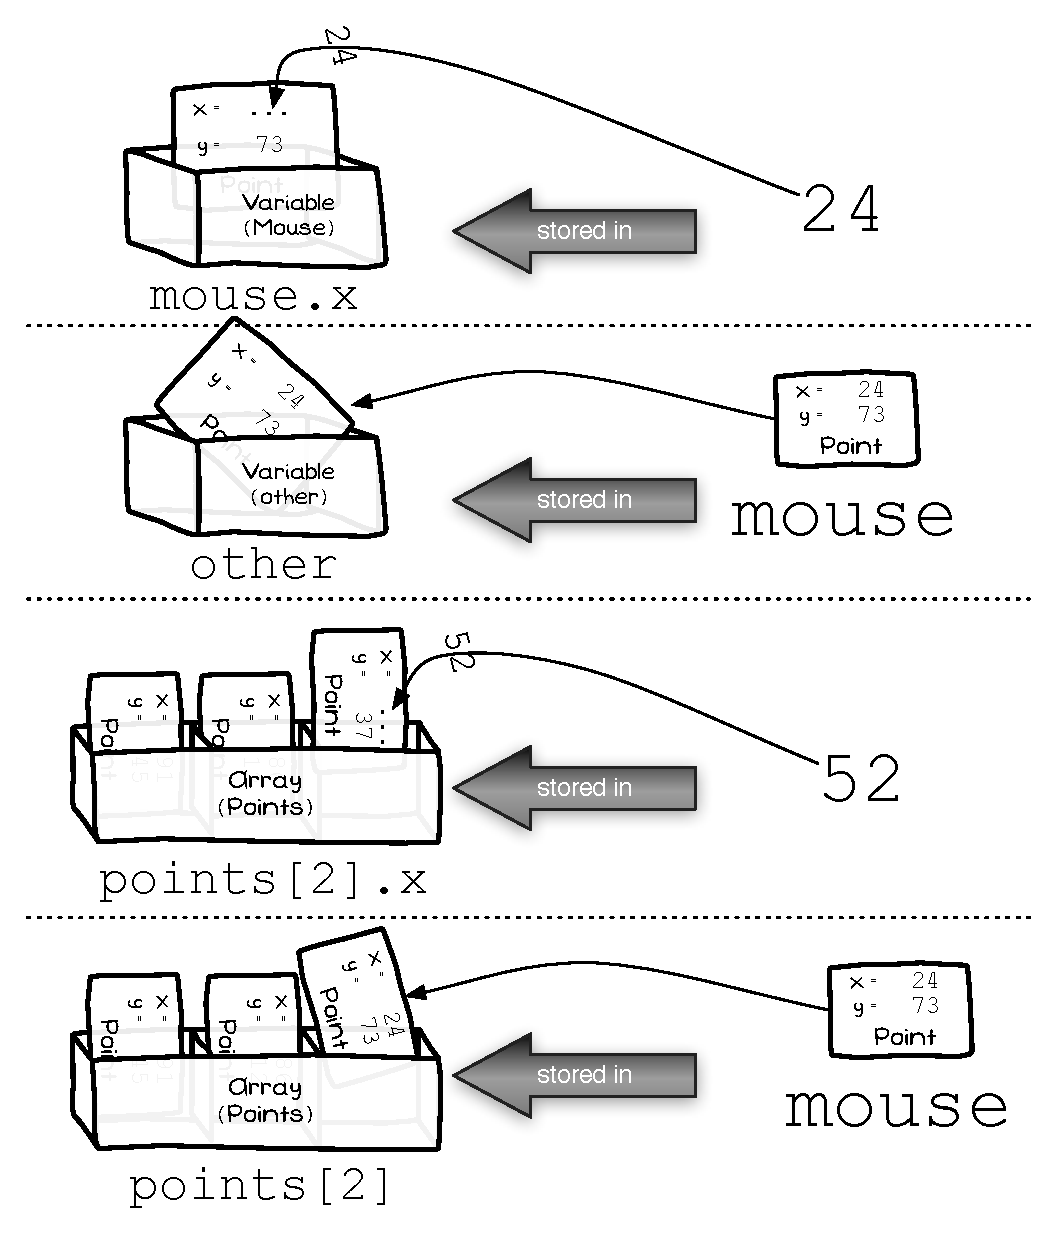
\includegraphics[width=0.8\textwidth]{./topics/type-decl/diagrams/RecordAssign} 
   \caption{You can assign an individual field or the entire record in one assignment statement}
   \label{fig:record-assign}
\end{figure}

\mynote{
\begin{itemize}
  \item The four examples from \ref{fig:record-assign} show the following:
  \begin{enumerate}
    \item You can assign a value to a field of a record. In this case 24 is assigned to \texttt{mouse.x}.
    \item A \texttt{Point} expression can be assigned to a \texttt{Point} variable. This copies the entire record into the Variable.
    \item It doesn't matter if the record is in an array, you can still assign a value to an record's fields.
    \item You can also assign an entire record into an element of an array.
  \end{enumerate}
  \item If the language allows arrays to be copied then you can also copy an entire array of records to a destination.
\end{itemize}
}

% subsubsection record_assignment (end)

\clearpage
\subsubsection{Union Assignment} % (fold)
\label{ssub:union_assignment}

The \nameref{ssub:union} is similar to a Record in that you can assign values to a union via its fields or by copying another union value into the variable or array element. The difference with the Union is that it has only a single value, with the different fields giving you different interpretations of that data.

\begin{figure}[h]
   \centering
   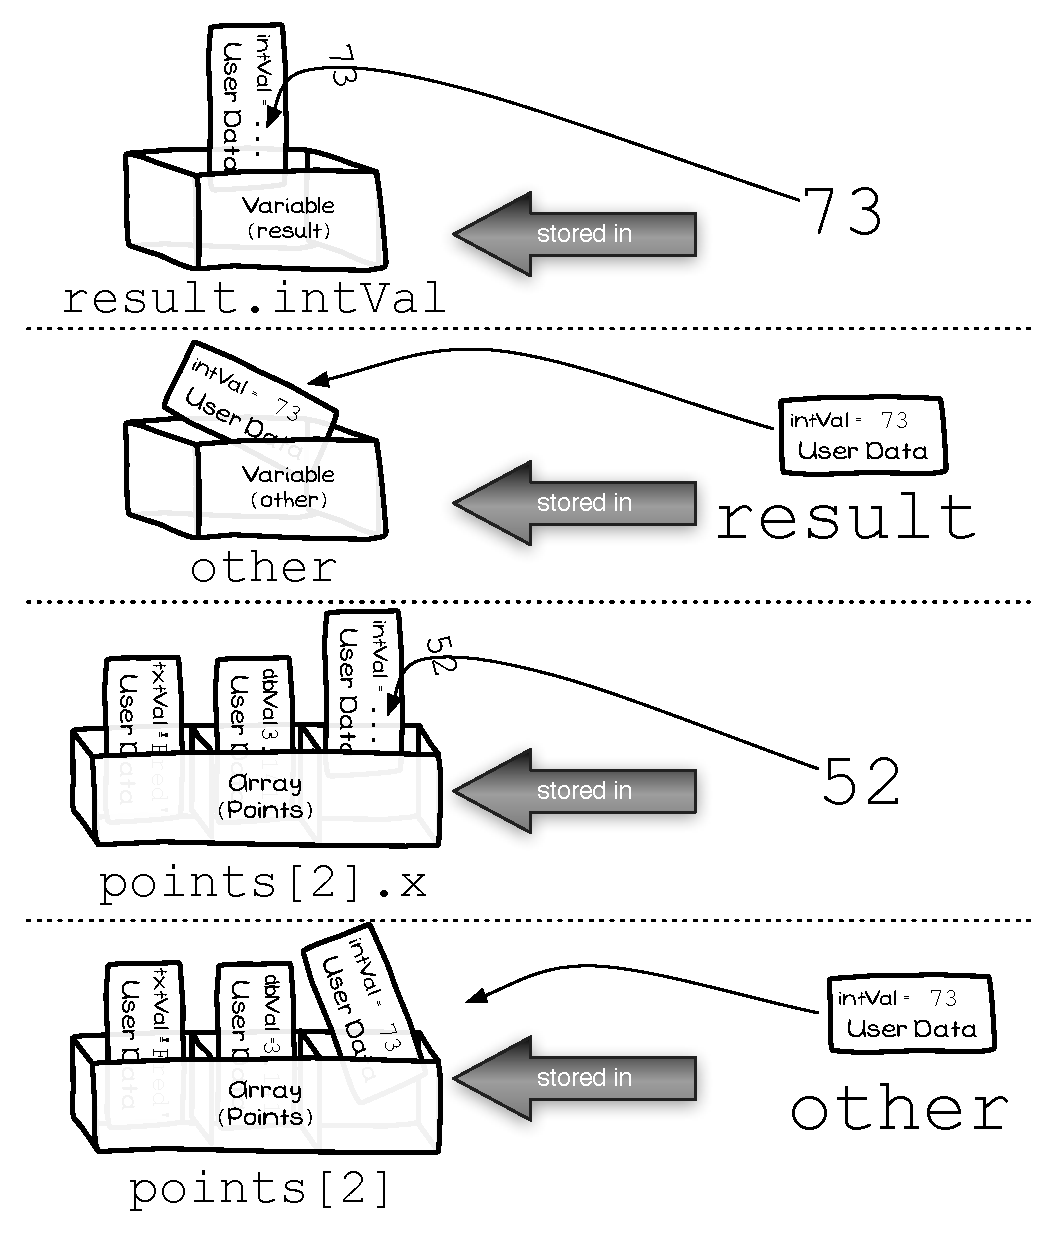
\includegraphics[width=0.8\textwidth]{./topics/type-decl/diagrams/UnionAssign} 
   \caption{You can assign an individual field or the entire union in one assignment statement}
   \label{fig:union-assign}
\end{figure}

\mynote{
\begin{itemize}
  \item The four examples from \ref{fig:union-assign} show the following:
  \begin{enumerate}
    \item You can assign a value to the fields of a Union. This overrides any value currently stored in the Variable.
    \item It is possible to copy an entire Union value in the assignment.
    \item This works in the same way with arrays, you can write a value to an Union.
    \item You can also copy an existing union value into an element.
  \end{enumerate}
  \item When accessing the data in a Union you are responsible for ensuring you read back the value you stored as it does not remember the kind of value you stored in the union.
\end{itemize}
}


% subsubsection union_assignment (end)

% subsection assignment_statement_with_fields_and_elements_ (end)